\section{System Model} \subsection{}
	
	\begin{frame}[fragile=singleslide]
	\frametitle{System Model}
	 
	Project consists of 4 packages:
		\begin{itemize}
			\item elements : deals with elements
			\item tool : offers important tools (e.g. read input)
			\item unificationProblem : treats the unification problem
			\item userInterfaces : allow user interfaces
		\end{itemize}
	
  \end{frame}	
		
%---------------------------------------------------------------

	\begin{frame}[fragile=singleslide]
	\frametitle{Package \texttt{elements}}
	
	\begin{figure}
		\centering
			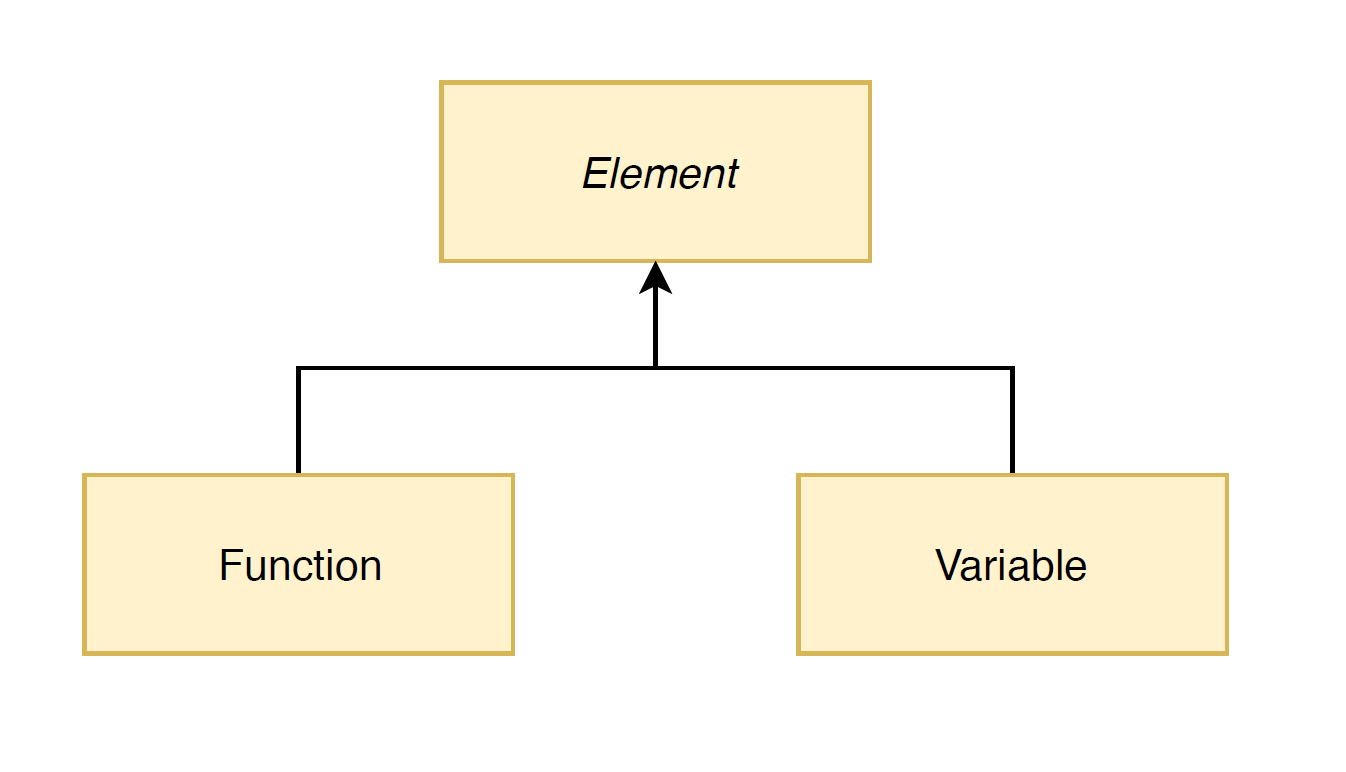
\includegraphics[width=8cm]{Bilder/elements.PNG}
		\label{fig:elements}
	\end{figure}
	
  \end{frame}	

%---------------------------------------------------------------

	\begin{frame}[fragile=singleslide]
	\frametitle{Package \texttt{tool}}
	 
	\begin{figure}
		\centering
			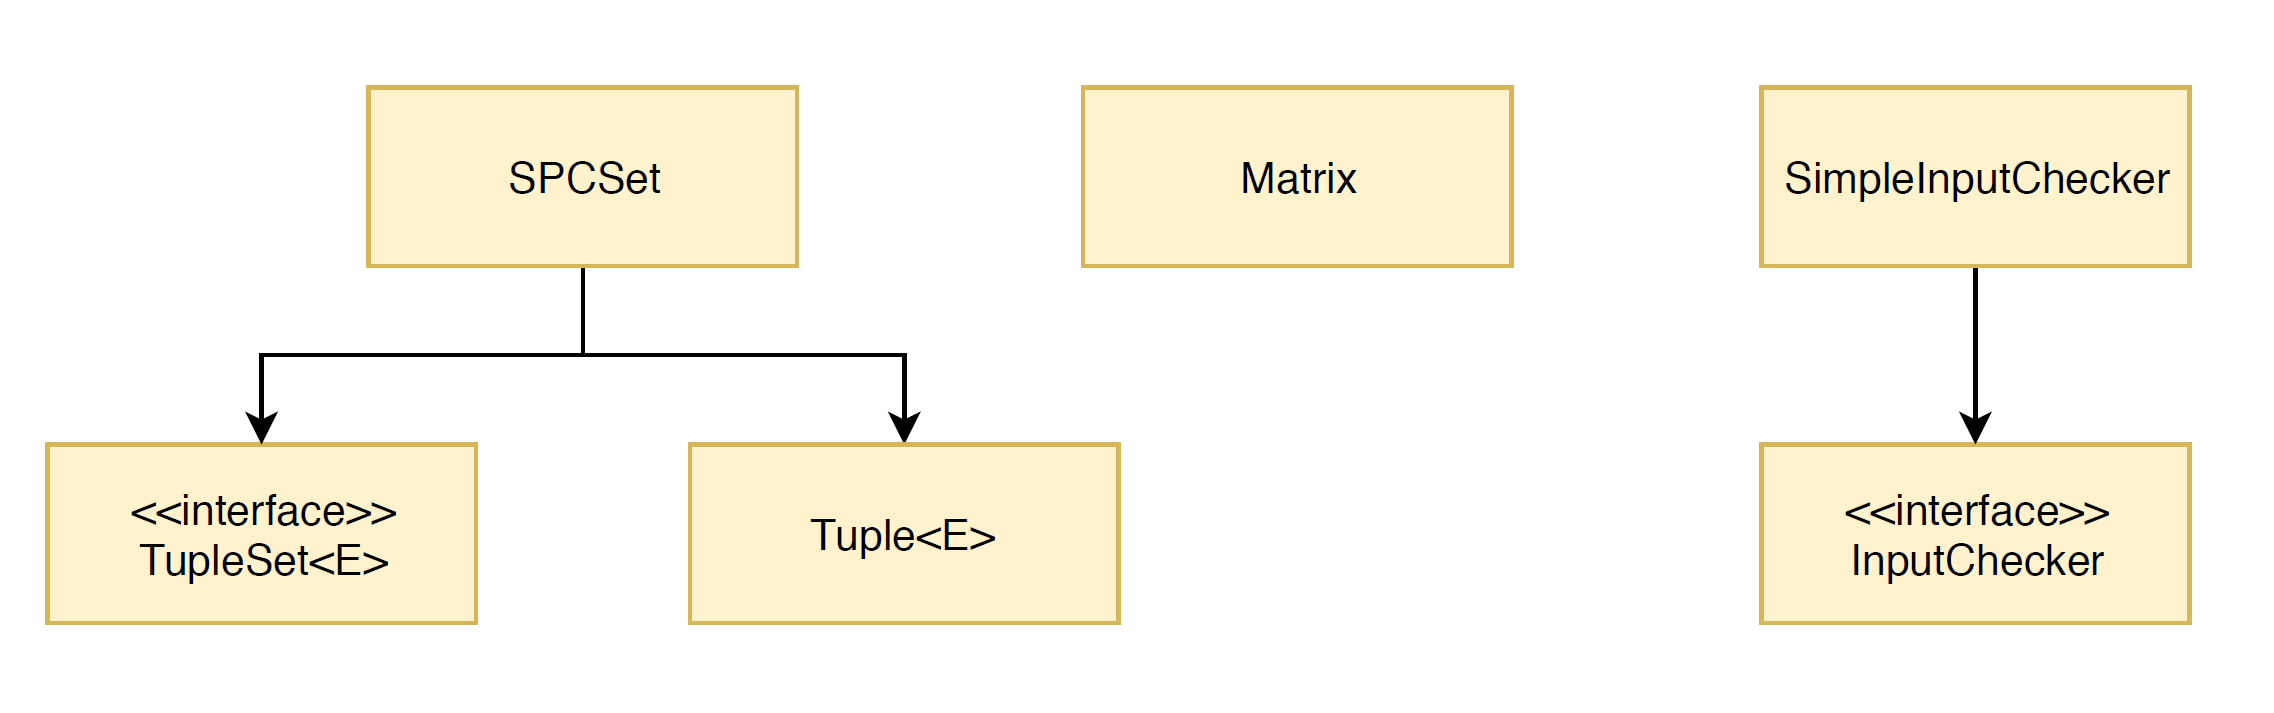
\includegraphics[width=11cm]{Bilder/tool.PNG}
		\label{fig:elements}
	\end{figure}
	
  \end{frame}	

%---------------------------------------------------------------

	\begin{frame}[fragile=singleslide]
	\frametitle{Package \texttt{unificationProblem}}
	 
	\begin{figure}
		\centering
			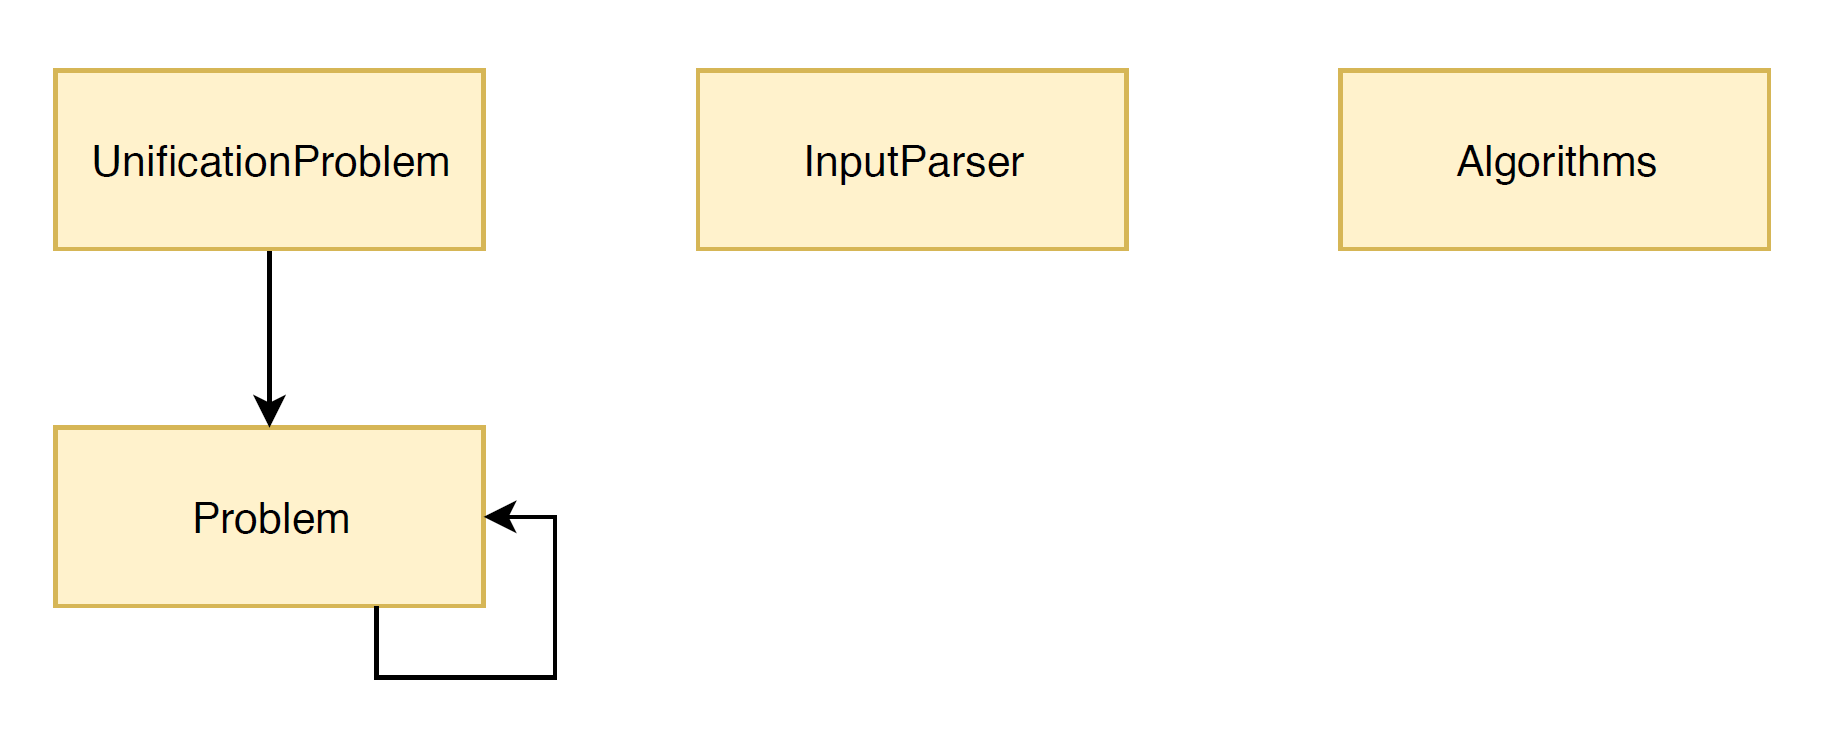
\includegraphics[width=11cm]{Bilder/unificationProblem.PNG}
		\label{fig:elements}
	\end{figure}
	
  \end{frame}	
	
%---------------------------------------------------------------
	
	\begin{frame}[fragile=singleslide]
	\frametitle{Package \texttt{userInterfaces}}
	 

	
  \end{frame}

%===============================================================
	\section{Workflow} \subsection{}
%===============================================================
	
		\begin{frame}[fragile=singleslide]
		\frametitle{Workflow}
		
		\begin{figure}
			\centering
				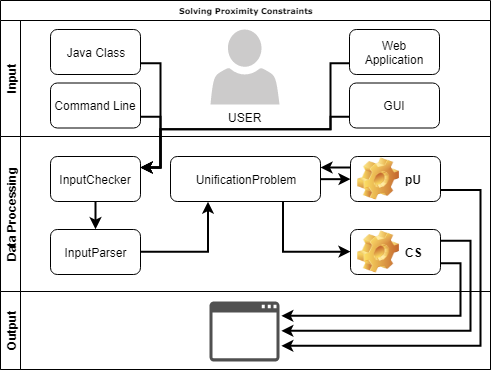
\includegraphics[width=8cm]{Bilder/WorkFlow.PNG}
			\label{fig:WorkFlow}
		\end{figure}
		
		\end{frame}

%---------------------------------------------------------------
